\chapter{Automa\c{c}\~ao DNS e Web (Parte II)}
\label{cap4}

\section{Enquadramento do cap\'{\i}tulo}

Este cap\'{\i}tulo d\'{a} continuidade \`a automa\c{c}\~ao DNS e Web, com foco em opera\c{c}\~oes de remo\c{c}\~ao controlada, manuten\c{c}\~ao e robustez operacional. S\~ao apresentados os pontos associados \`a elimina\c{c}\~ao de configura\c{c}\~oes (Quest\~ao 6) e \`as melhorias de administra\c{c}\~ao e seguran\c{c}a (Quest\~ao 8), ficando este cap\'{\i}tulo preparado para integrar tamb\'{e}m o ponto P13 e restantes refor\c{c}os de seguran\c{c}a.
\section{Quest\~ao 6: eliminac\~ao de zonas master, VirtualHosts e zonas reverse}
\label{sec:q6}

\subsection{Objetivo}

A Quest\~ao 6 introduz a capacidade de remo\c{c}\~ao autom\'atica de elementos previamente criados nas quest\~oes anteriores. Em vez de se limitar \`a cria\c{c}\~ao de configura\c{c}\~oes, a aplica\c{c}\~ao passa tamb\'em a suportar opera\c{c}\~oes de elimina\c{c}\~ao controlada de zonas DNS \textit{forward}, VirtualHosts Apache e zonas DNS \textit{reverse}.

Esta funcionalidade completa o ciclo de administra\c{c}\~ao, permitindo criar e remover configura\c{c}\~oes de forma coerente, sem deixar entradas residuais nos servi\c{c}os.

\subsection{Implementa\c{c}\~ao do script \texttt{q6\_remover.sh}}

O script \texttt{q6\_remover.sh} concentra num \'unico ponto as opera\c{c}\~oes de remo\c{c}\~ao relacionadas com DNS e Apache. A l\'ogica principal cobre tr\^es opera\c{c}\~oes:

\begin{enumerate}
    \item elimina\c{c}\~ao de zonas master \textit{forward};
    \item elimina\c{c}\~ao de VirtualHosts Apache;
    \item elimina\c{c}\~ao de zonas \textit{reverse}.
\end{enumerate}

\begin{lstlisting}[language=bash,caption={Estrutura base do script}]
CONFZONES="/etc/named/zones.conf"
ZONEDIR="/var/named"
HTTPD_CONF_DIR="/etc/httpd/conf.d"
WEBROOT_BASE="/var/www"
\end{lstlisting}

Estas vari\'aveis definem de forma expl\'icita os locais de configura\c{c}\~ao e dados onde o script atua.

\begin{lstlisting}[language=bash,caption={Remocao de blocos de zona no zones.conf}]
remover_bloco_zona() {
    local nomezona="$1"

    awk -v zona="$nomezona" '
    BEGIN {skip=0}
    $0 ~ "^[[:space:]]*zone \""zona"\"" {skip=1; next}
    skip==1 && $0 ~ /^[[:space:]]*};[[:space:]]*$/ {skip=0; next}
    skip==0 {print}
    ' "$CONFZONES" > /tmp/zones.conf.new && mv /tmp/zones.conf.new "$CONFZONES"
}
\end{lstlisting}

Esta fun\c{c}\~ao \'{e} o n\'ucleo da remo\c{c}\~ao DNS, pois elimina o bloco completo da zona no \texttt{zones.conf}, e n\~ao apenas uma linha isolada.

\begin{lstlisting}[language=bash,caption={Eliminacao de zonas master forward}]
eliminar_zona_forward() {
    read -p "Dominio da zona master a eliminar: " DOMINIO
    ZONEFILE="$ZONEDIR/${DOMINIO}.zone"

    if grep -q "zone \"$DOMINIO\"" "$CONFZONES"; then
        remover_bloco_zona "$DOMINIO"
    fi

    [ -f "$ZONEFILE" ] && rm -f "$ZONEFILE"

    named-checkconf || { echo "Erro na configuracao DNS."; exit 1; }
    systemctl restart named
}
\end{lstlisting}

Nesta opera\c{c}\~ao, a remo\c{c}\~ao s\'o fica completa quando s\~ao eliminados tanto o bloco da zona no \texttt{zones.conf} como o ficheiro \texttt{.zone} em \texttt{/var/named}.

\begin{lstlisting}[language=bash,caption={Eliminacao de VirtualHosts Apache}]
eliminar_virtualhost() {
    read -p "Dominio do VirtualHost a eliminar: " DOMINIO

    VHOSTFILE="$HTTPD_CONF_DIR/${DOMINIO}.conf"
    WEBROOT="$WEBROOT_BASE/${DOMINIO}"

    [ -f "$VHOSTFILE" ] && rm -f "$VHOSTFILE"

    read -p "Deseja apagar tambem a pasta web $WEBROOT ? (s/n): " OP
    if [ "$OP" = "s" ] || [ "$OP" = "S" ]; then
        [ -d "$WEBROOT" ] && rm -rf "$WEBROOT"
    fi

    httpd -t || { echo "Erro na configuracao Apache."; exit 1; }
    systemctl restart httpd
}
\end{lstlisting}

Este bloco remove o ficheiro de VirtualHost e, opcionalmente, a diretoria Web correspondente, permitindo uma remo\c{c}\~ao parcial ou completa conforme a necessidade.

\begin{lstlisting}[language=bash,caption={Eliminacao de zonas reverse}]
eliminar_zona_reverse() {
    read -p "Zona reverse a eliminar (ex: 2.50.10.in-addr.arpa): " REVZONE

    REVBASE=$(echo "$REVZONE" | sed 's/\.in-addr\.arpa//')
    REVFILE="$ZONEDIR/${REVBASE}.rev"

    if grep -q "zone \"$REVZONE\"" "$CONFZONES"; then
        remover_bloco_zona "$REVZONE"
    fi

    [ -f "$REVFILE" ] && rm -f "$REVFILE"

    named-checkconf || { echo "Erro na configuracao DNS."; exit 1; }
    systemctl restart named
}
\end{lstlisting}

Na remo\c{c}\~ao \textit{reverse}, o script converte primeiro a zona no formato \texttt{in-addr.arpa} para o nome base do ficheiro \texttt{.rev}, e depois aplica a mesma l\'ogica de consist\^encia usada nas zonas \textit{forward}.

\begin{lstlisting}[language=bash,caption={Menu de remocao}]
menu() {
    echo
    echo "===== MENU REMOCAO ====="
    echo "1 - Eliminar zona master (forward)"
    echo "2 - Eliminar VirtualHost"
    echo "3 - Eliminar zona reverse"
    echo "0 - Sair"
    echo
    read -p "Opcao: " OP

    case $OP in
        1) eliminar_zona_forward ;;
        2) eliminar_virtualhost ;;
        3) eliminar_zona_reverse ;;
        0) exit 0 ;;
        *) echo "Opcao invalida." ;;
    esac
}
\end{lstlisting}

O menu simplifica a utiliza\c{c}\~ao e centraliza as opera\c{c}\~oes de remo\c{c}\~ao num \'unico ponto.

\subsection{Valida\c{c}\~ao funcional}

A valida\c{c}\~ao foi realizada com execu\c{c}\~ao do script e verifica\c{c}\~ao dos ficheiros de configura\c{c}\~ao antes e depois das remo\c{c}\~oes.

\begin{lstlisting}[language=bash,caption={Execucao do script}]
chmod +x /root/projeto/q6_remover.sh
/root/projeto/q6_remover.sh
\end{lstlisting}

Foram testadas as tr\^es op\c{c}\~oes do menu: elimina\c{c}\~ao de zona \textit{forward}, elimina\c{c}\~ao de VirtualHost e elimina\c{c}\~ao de zona \textit{reverse}.

\begin{lstlisting}[language=bash,caption={Verificacao da remocao de VirtualHosts}]
ls /etc/httpd/conf.d
ls /var/www
httpd -t
\end{lstlisting}

\begin{lstlisting}[language=bash,caption={Verificacao da remocao de zonas DNS}]
cat /etc/named/zones.conf
ls /var/named
named-checkconf
\end{lstlisting}

Os testes confirmaram a remo\c{c}\~ao correta dos elementos selecionados e a manuten\c{c}\~ao da validade das configura\c{c}\~oes de DNS e Apache ap\'os cada opera\c{c}\~ao.

\subsection{Evid\^encias visuais da Quest\~ao 6}

\begin{figure}[!htbp]
\centering
\IfFileExists{figuras/q6_pre_www.png}{
  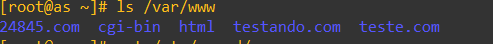
\includegraphics[width=0.78\textwidth,height=0.72\textheight,keepaspectratio]{figuras/q6_pre_www.png}
}{
  \fbox{\parbox{0.9\textwidth}{Inserir screenshot do estado inicial de \texttt{/var/www}.}}
}
\caption{Estado inicial da diretoria \texttt{/var/www}}
\label{fig:q6-pre-www}
\end{figure}

\begin{figure}[!htbp]
\centering
\IfFileExists{figuras/q6_pre_httpd_conf.png}{
  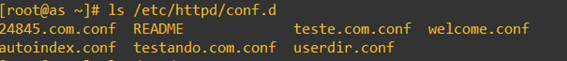
\includegraphics[width=0.78\textwidth,height=0.72\textheight,keepaspectratio]{figuras/q6_pre_httpd_conf.png}
}{
  \fbox{\parbox{0.9\textwidth}{Inserir screenshot do estado inicial de \texttt{/etc/httpd/conf.d}.}}
}
\caption{Estado inicial dos VirtualHosts em \texttt{/etc/httpd/conf.d}}
\label{fig:q6-pre-httpd}
\end{figure}

\begin{figure}[!htbp]
\centering
\IfFileExists{figuras/q6_pre_zones_conf.png}{
  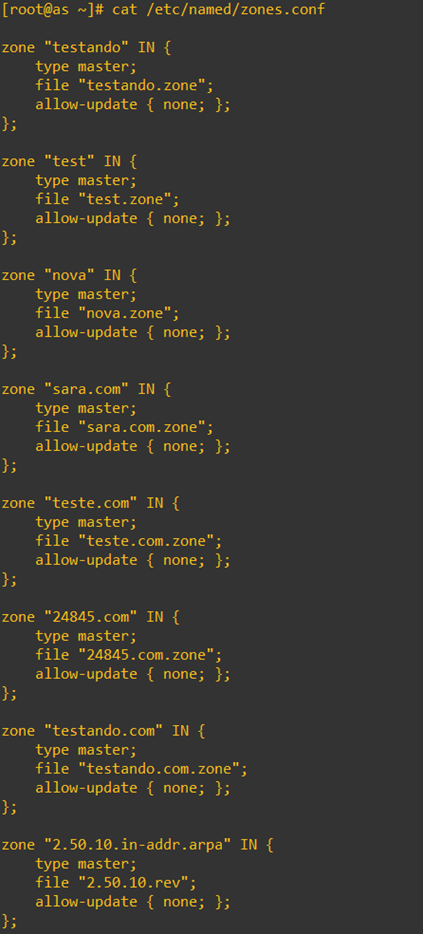
\includegraphics[width=0.78\textwidth,height=0.72\textheight,keepaspectratio]{figuras/q6_pre_zones_conf.png}
}{
  \fbox{\parbox{0.9\textwidth}{Inserir screenshot inicial de \texttt{/etc/named/zones.conf}.}}
}
\caption{Estado inicial do ficheiro \texttt{zones.conf}}
\label{fig:q6-pre-zones}
\end{figure}

\begin{figure}[!htbp]
\centering
\IfFileExists{figuras/q6_exec_forward.png}{
  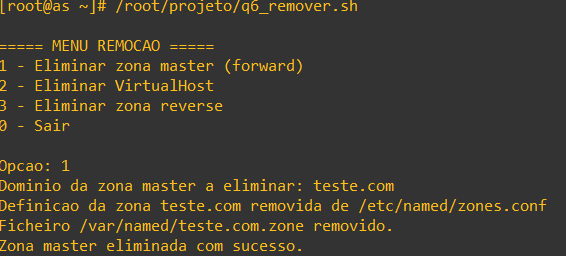
\includegraphics[width=0.78\textwidth,height=0.72\textheight,keepaspectratio]{figuras/q6_exec_forward.png}
}{
  \fbox{\parbox{0.9\textwidth}{Inserir screenshot da remocao de zona master (opcao 1).}}
}
\caption{Execucao da opcao de remocao de zona master forward}
\label{fig:q6-exec-forward}
\end{figure}

\begin{figure}[!htbp]
\centering
\IfFileExists{figuras/q6_exec_vhost.png}{
  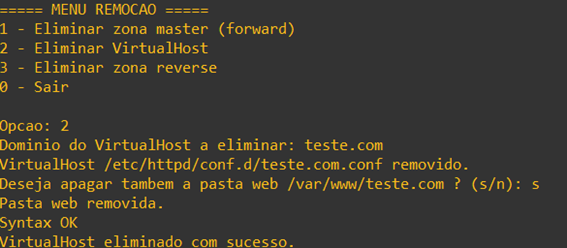
\includegraphics[width=0.78\textwidth,height=0.72\textheight,keepaspectratio]{figuras/q6_exec_vhost.png}
}{
  \fbox{\parbox{0.9\textwidth}{Inserir screenshot da remocao de VirtualHost (opcao 2).}}
}
\caption{Execucao da opcao de remocao de VirtualHost}
\label{fig:q6-exec-vhost}
\end{figure}

\begin{figure}[!htbp]
\centering
\IfFileExists{figuras/q6_exec_reverse.png}{
  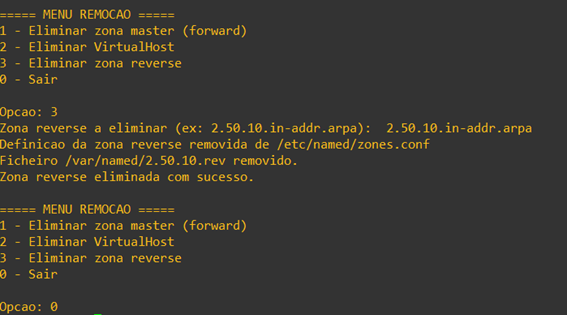
\includegraphics[width=0.78\textwidth,height=0.72\textheight,keepaspectratio]{figuras/q6_exec_reverse.png}
}{
  \fbox{\parbox{0.9\textwidth}{Inserir screenshot da remocao de zona reverse (opcao 3).}}
}
\caption{Execucao da opcao de remocao de zona reverse}
\label{fig:q6-exec-reverse}
\end{figure}

\begin{figure}[!htbp]
\centering
\IfFileExists{figuras/q6_pos_httpd_www.png}{
  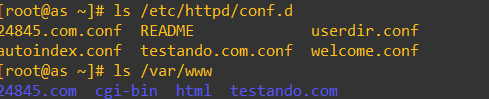
\includegraphics[width=0.78\textwidth,height=0.72\textheight,keepaspectratio]{figuras/q6_pos_httpd_www.png}
}{
  \fbox{\parbox{0.9\textwidth}{Inserir screenshot do estado final de \texttt{/etc/httpd/conf.d} e \texttt{/var/www}.}}
}
\caption{Estado final das estruturas Apache ap\'os remo\c{c}\~ao}
\label{fig:q6-pos-httpd}
\end{figure}

\begin{figure}[!htbp]
\centering
\IfFileExists{figuras/q6_pos_named.png}{
  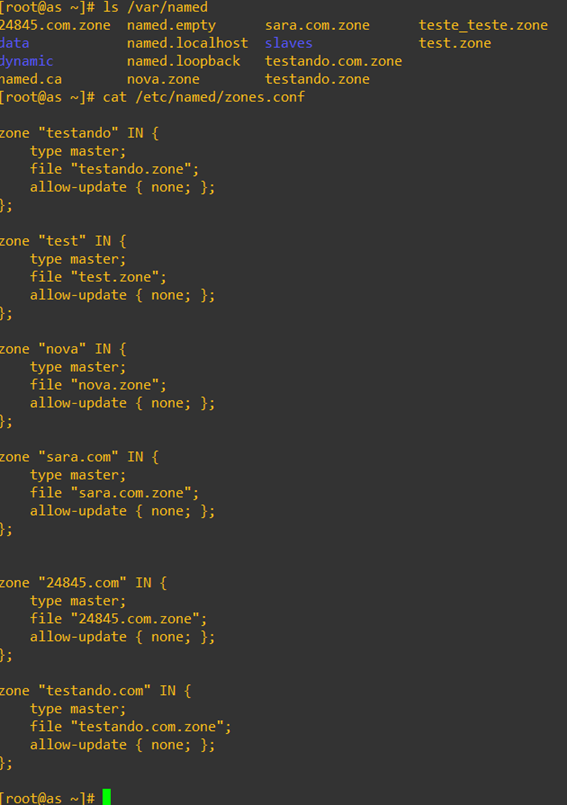
\includegraphics[width=0.78\textwidth,height=0.72\textheight,keepaspectratio]{figuras/q6_pos_named.png}
}{
  \fbox{\parbox{0.9\textwidth}{Inserir screenshot do estado final de \texttt{/var/named} e \texttt{zones.conf}.}}
}
\caption{Estado final das estruturas DNS ap\'os remo\c{c}\~ao}
\label{fig:q6-pos-named}
\end{figure}

\clearpage
\section{Quest\~ao 8: melhorias ao funcionamento da aplica\c{c}\~ao DNS}
\label{sec:q8}

\subsection{Objetivo}

A Quest\~ao 8 teve como finalidade refor\c{c}ar a aplica\c{c}\~ao desenvolvida nos pontos anteriores, introduzindo melhorias orientadas para manuten\c{c}\~ao, seguran\c{c}a operacional e robustez da configura\c{c}\~ao DNS. Em vez de acrescentar apenas uma fun\c{c}\~ao isolada, esta etapa evolui a administra\c{c}\~ao das zonas para um modelo mais seguro e mais adequado a utiliza\c{c}\~ao continuada.

As melhorias implementadas incidiram em cinco aspetos principais:
\begin{enumerate}
    \item atualiza\c{c}\~ao de registos DNS em zonas existentes;
    \item cria\c{c}\~ao autom\'atica de backups antes de altera\c{c}\~oes;
    \item reposi\c{c}\~ao da configura\c{c}\~ao anterior em caso de falha;
    \item registo das opera\c{c}\~oes em ficheiro de log;
    \item integra\c{c}\~ao das rotinas de manuten\c{c}\~ao num menu \'unico.
\end{enumerate}

\subsection{Implementa\c{c}\~ao do script \texttt{q8\_melhorias\_dns.sh}}

O script \texttt{q8\_melhorias\_dns.sh} funciona como uma camada de manuten\c{c}\~ao sobre as zonas j\'a criadas, acrescentando mecanismos de controlo que n\~ao existiam nas vers\~oes anteriores.

\begin{lstlisting}[language=bash,caption={Estrutura base, log e diretoria de backups}]
MAINCONF="/etc/named.conf"
CONFZONES="/etc/named/zones.conf"
ZONEDIR="/var/named"
LOGFILE="/var/log/projeto_dns.log"
BACKUPDIR="/root/projeto/backups_dns"

mkdir -p "$BACKUPDIR"
\end{lstlisting}

Com este bloco, a manuten\c{c}\~ao passa a ter rastreabilidade (\texttt{LOGFILE}) e recupera\c{c}\~ao (\texttt{BACKUPDIR}).

\begin{lstlisting}[language=bash,caption={Registo em log e backup automatico}]
regista_log() {
    echo "$(date '+%Y-%m-%d %H:%M:%S') - $1" >> "$LOGFILE"
}

backup_ficheiro() {
    local ficheiro="$1"
    if [ -f "$ficheiro" ]; then
        cp "$ficheiro" "$BACKUPDIR/$(basename "$ficheiro").bak.$(date +%Y%m%d%H%M%S)"
    fi
}
\end{lstlisting}

Estas fun\c{c}\~oes garantem historial das opera\c{c}\~oes e c\'opia de seguran\c{c}a antes de qualquer altera\c{c}\~ao ao ficheiro de zona.

\begin{lstlisting}[language=bash,caption={Validacao com rollback automatico}]
valida_e_aplica() {
    local dominio="$1"
    local ficheiro="$2"
    local tmpbackup="$3"

    named-checkconf >/dev/null 2>&1 || {
        regista_log "ERRO: named-checkconf falhou"
        [ -f "$tmpbackup" ] && cp "$tmpbackup" "$ficheiro"
        return 1
    }

    named-checkzone "$dominio" "$ficheiro" >/dev/null 2>&1 || {
        regista_log "ERRO: named-checkzone falhou para $dominio"
        [ -f "$tmpbackup" ] && cp "$tmpbackup" "$ficheiro"
        return 1
    }

    systemctl restart named || {
        regista_log "ERRO: restart do named falhou"
        [ -f "$tmpbackup" ] && cp "$tmpbackup" "$ficheiro"
        return 1
    }

    return 0
}
\end{lstlisting}

Este bloco introduz rollback autom\'atico: se a valida\c{c}\~ao falhar, o ficheiro volta ao estado anterior.

\begin{lstlisting}[language=bash,caption={Listagem de zonas e registos}]
listar_zonas() {
    grep '^zone "' "$CONFZONES" 2>/dev/null | awk -F'"' '{print $2}'
}

listar_registos() {
    read -p "Dominio: " DOMINIO
    ZONEFILE="$ZONEDIR/${DOMINIO}.zone"

    [ ! -f "$ZONEFILE" ] && { echo "Erro: zona nao encontrada."; return; }
    grep -E 'IN[[:space:]]+(A|MX|PTR)' "$ZONEFILE"
}
\end{lstlisting}

Estas rotinas permitem consultar o estado atual antes de alterar a zona, reduzindo erros operacionais.

\begin{lstlisting}[language=bash,caption={Adicao de registos com protecao adicional}]
adicionar_registo_a() {
    read -p "Dominio: " DOMINIO
    read -p "Host (ex: www, mail, ftp, @): " HOST
    read -p "IP: " IP

    ZONEFILE="$ZONEDIR/${DOMINIO}.zone"
    [ ! -f "$ZONEFILE" ] && { echo "Erro: zona nao encontrada."; return; }
    grep -q "^$HOST[[:space:]].*IN[[:space:]]\+A" "$ZONEFILE" && {
        echo "Erro: ja existe registo A para esse host."; return;
    }

    backup_ficheiro "$ZONEFILE"
    TMPBACKUP="/tmp/$(basename "$ZONEFILE").pre"
    cp "$ZONEFILE" "$TMPBACKUP"

    echo "$HOST    IN    A    $IP" >> "$ZONEFILE"
    atualiza_serial "$ZONEFILE"

    valida_e_aplica "$DOMINIO" "$ZONEFILE" "$TMPBACKUP" && \
    regista_log "Registo A adicionado em $DOMINIO: $HOST -> $IP"

    rm -f "$TMPBACKUP"
}
\end{lstlisting}

O fluxo aplicado aqui (backup, altera\c{c}\~ao, valida\c{c}\~ao, log) foi mantido tamb\'em nas opera\c{c}\~oes de atualiza\c{c}\~ao e remo\c{c}\~ao.

\begin{lstlisting}[language=bash,caption={Atualizacao de registos existentes}]
atualizar_registo_a() {
    read -p "Dominio: " DOMINIO
    read -p "Host do registo A a atualizar: " HOST
    read -p "Novo IP: " NOVOIP

    ZONEFILE="$ZONEDIR/${DOMINIO}.zone"
    [ ! -f "$ZONEFILE" ] && { echo "Erro: zona nao encontrada."; return; }
    grep -q "^$HOST[[:space:]].*IN[[:space:]]\+A" "$ZONEFILE" || {
        echo "Erro: registo A nao encontrado."; return;
    }

    backup_ficheiro "$ZONEFILE"
    TMPBACKUP="/tmp/$(basename "$ZONEFILE").pre"
    cp "$ZONEFILE" "$TMPBACKUP"

    sed -i "/^$HOST[[:space:]].*IN[[:space:]]\+A/c\\$HOST    IN    A    $NOVOIP" "$ZONEFILE"
    atualiza_serial "$ZONEFILE"

    valida_e_aplica "$DOMINIO" "$ZONEFILE" "$TMPBACKUP" && \
    regista_log "Registo A atualizado em $DOMINIO: $HOST -> $NOVOIP"

    rm -f "$TMPBACKUP"
}
\end{lstlisting}

\begin{lstlisting}[language=bash,caption={Remocao de registos com validacao e recuperacao}]
remover_registo() {
    read -p "Dominio: " DOMINIO
    read -p "Host a remover: " HOST
    read -p "Tipo de registo (A/MX/PTR): " TIPO

    ZONEFILE="$ZONEDIR/${DOMINIO}.zone"
    [ ! -f "$ZONEFILE" ] && { echo "Erro: zona nao encontrada."; return; }

    backup_ficheiro "$ZONEFILE"
    TMPBACKUP="/tmp/$(basename "$ZONEFILE").pre"
    cp "$ZONEFILE" "$TMPBACKUP"

    grep -v "^$HOST[[:space:]].*IN[[:space:]]\+$TIPO" "$ZONEFILE" > /tmp/zone.new
    mv /tmp/zone.new "$ZONEFILE"
    atualiza_serial "$ZONEFILE"

    valida_e_aplica "$DOMINIO" "$ZONEFILE" "$TMPBACKUP" && \
    regista_log "Registo removido em $DOMINIO: $HOST $TIPO"

    rm -f "$TMPBACKUP"
}
\end{lstlisting}

\begin{lstlisting}[language=bash,caption={Menu unificado de manutencao DNS}]
menu() {
    echo "===== MELHORIAS DNS - PONTO 8 ====="
    echo "1 - Listar zonas"
    echo "2 - Listar registos de uma zona"
    echo "3 - Adicionar registo A"
    echo "4 - Adicionar registo MX"
    echo "5 - Atualizar registo A"
    echo "6 - Atualizar registo MX"
    echo "7 - Remover registo"
    echo "8 - Ver log"
    echo "0 - Sair"
}
\end{lstlisting}

O menu centraliza as opera\c{c}\~oes e torna a manuten\c{c}\~ao mais simples no dia a dia.

\subsection{Valida\c{c}\~ao funcional}

A valida\c{c}\~ao foi feita com execu\c{c}\~ao do script e demonstra\c{c}\~ao das opera\c{c}\~oes principais: listagem, adi\c{c}\~ao, atualiza\c{c}\~ao, remo\c{c}\~ao, consulta de log e verifica\c{c}\~ao dos backups.

\begin{lstlisting}[language=bash,caption={Execucao do script}]
chmod +x /root/projeto/q8_melhorias_dns.sh
/root/projeto/q8_melhorias_dns.sh
\end{lstlisting}

\begin{lstlisting}[language=bash,caption={Verificacao do log das operacoes}]
tail -n 30 /var/log/projeto_dns.log
\end{lstlisting}

\begin{lstlisting}[language=bash,caption={Verificacao dos backups gerados}]
ls -l /root/projeto/backups_dns
\end{lstlisting}

Nos testes realizados, as opera\c{c}\~oes foram registadas corretamente e os backups foram gerados com carimbo temporal antes de cada altera\c{c}\~ao. Foi ainda poss\'ivel confirmar a manuten\c{c}\~ao de registos sem edi\c{c}\~ao manual do ficheiro de zona.

\subsection{Evid\^encias visuais da Quest\~ao 8}

\begin{figure}[!htbp]
\centering
\IfFileExists{figuras/q8_menu_listagem.png}{
  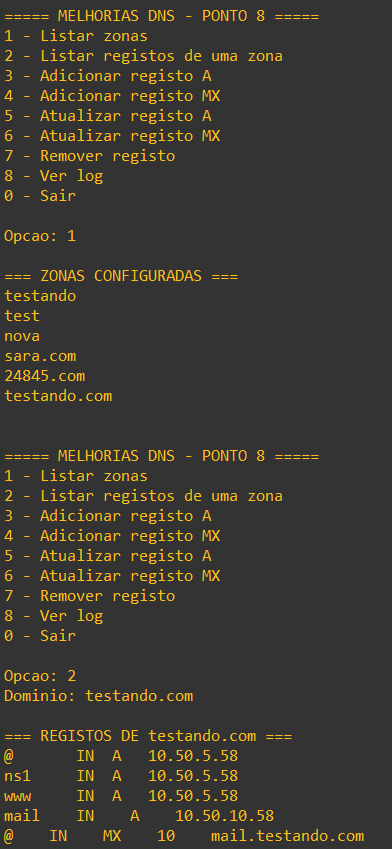
\includegraphics[width=0.78\textwidth,height=0.72\textheight,keepaspectratio]{figuras/q8_menu_listagem.png}
}{
  \fbox{\parbox{0.9\textwidth}{Inserir screenshot do menu da Quest\~ao 8 e listagem inicial de zonas/registos.}}
}
\caption{Menu da Quest\~ao 8 e listagem inicial de zonas e registos}
\label{fig:q8-menu-listagem}
\end{figure}

\begin{figure}[!htbp]
\centering
\IfFileExists{figuras/q8_add_a_mx.png}{
  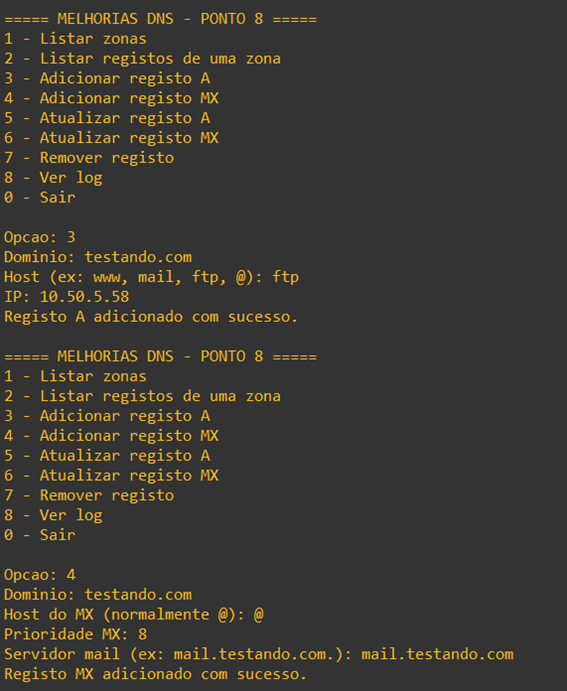
\includegraphics[width=0.78\textwidth,height=0.72\textheight,keepaspectratio]{figuras/q8_add_a_mx.png}
}{
  \fbox{\parbox{0.9\textwidth}{Inserir screenshot da adi\c{c}\~ao de registos A e MX.}}
}
\caption{Adi\c{c}\~ao de registos A e MX}
\label{fig:q8-add}
\end{figure}

\begin{figure}[!htbp]
\centering
\IfFileExists{figuras/q8_update_a_mx.png}{
  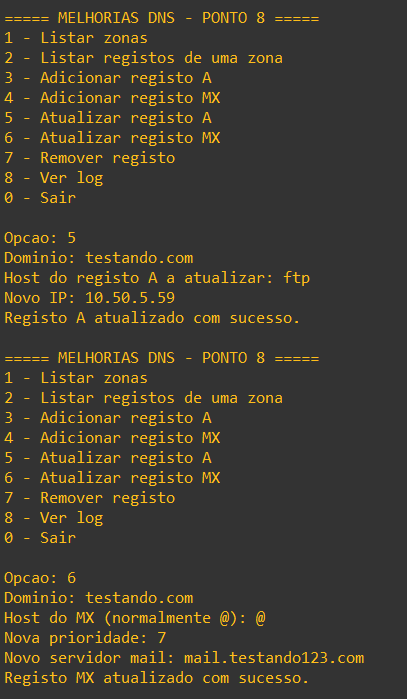
\includegraphics[width=0.78\textwidth,height=0.72\textheight,keepaspectratio]{figuras/q8_update_a_mx.png}
}{
  \fbox{\parbox{0.9\textwidth}{Inserir screenshot da atualiza\c{c}\~ao de registos A e MX.}}
}
\caption{Atualiza\c{c}\~ao de registos A e MX}
\label{fig:q8-update}
\end{figure}

\begin{figure}[!htbp]
\centering
\IfFileExists{figuras/q8_remove_log.png}{
  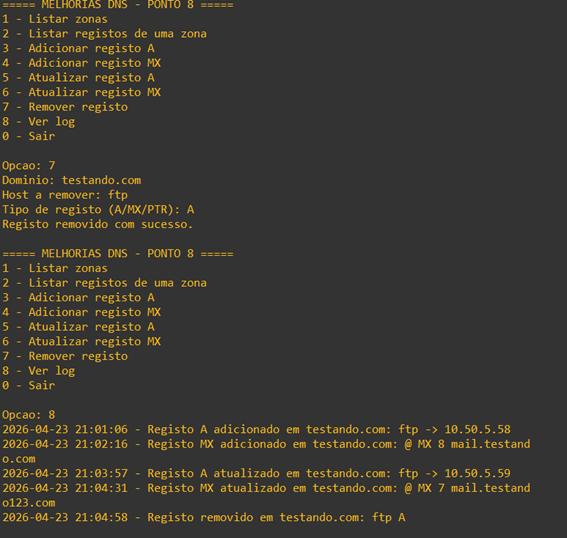
\includegraphics[width=0.78\textwidth,height=0.72\textheight,keepaspectratio]{figuras/q8_remove_log.png}
}{
  \fbox{\parbox{0.9\textwidth}{Inserir screenshot da remo\c{c}\~ao de registo e visualiza\c{c}\~ao do log.}}
}
\caption{Remo\c{c}\~ao de registos e consulta do log}
\label{fig:q8-remove-log}
\end{figure}

\begin{figure}[!htbp]
\centering
\IfFileExists{figuras/q8_listagem_final.png}{
  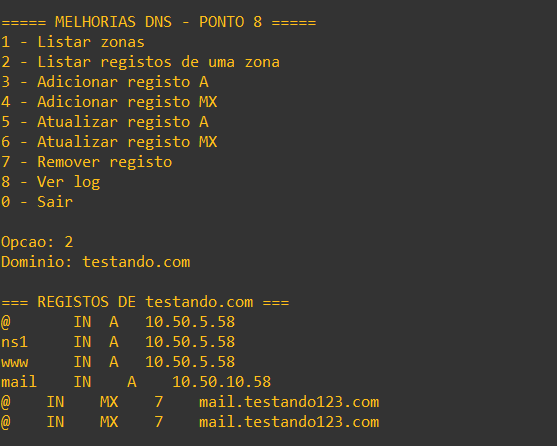
\includegraphics[width=0.78\textwidth,height=0.72\textheight,keepaspectratio]{figuras/q8_listagem_final.png}
}{
  \fbox{\parbox{0.9\textwidth}{Inserir screenshot da listagem final de registos no dom\'{\i}nio de teste.}}
}
\caption{Estado final dos registos ap\'os as opera\c{c}\~oes de manuten\c{c}\~ao}
\label{fig:q8-final}
\end{figure}

\clearpage
\section{Quest\~ao 13: cria\c{c}\~ao e gest\~ao de blacklist de dom\'inios no servidor DNS}
\label{sec:q13}

\subsection{Objetivo}

A Quest\~ao 13 teve como objetivo implementar um mecanismo de \textit{blacklist} DNS, fazendo com que dom\'inios selecionados deixem de resolver para os endere\c{c}os reais e passem a responder sempre para um IP fixo definido localmente. Para cumprir o enunciado, a solu\c{c}\~ao inclui:
\begin{enumerate}
    \item prepara\c{c}\~ao da infraestrutura de \textit{response policy} no BIND;
    \item inser\c{c}\~ao de dom\'inios na blacklist;
    \item remo\c{c}\~ao e listagem dos dom\'inios bloqueados.
\end{enumerate}

\subsection{Implementa\c{c}\~ao do script \texttt{q13\_blacklist\_dns.sh}}

O script implementa a blacklist atrav\'es de uma zona de pol\'itica de resposta (\texttt{RPZ}), designada \texttt{rpz.local}.

\begin{lstlisting}[language=bash,caption={Estrutura base da blacklist DNS}]
MAINCONF="/etc/named.conf"
CONFZONES="/etc/named/zones.conf"
RPZ_ZONE="rpz.local"
RPZ_FILE="/var/named/rpz.local.zone"
FIXED_IP="10.50.2.214"
\end{lstlisting}

Esta base separa a blacklist da configura\c{c}\~ao normal das zonas forward, mantendo a administra\c{c}\~ao mais organizada.

\begin{lstlisting}[language=bash,caption={Garantia de integracao com a configuracao DNS}]
garante_zones_conf() {
    touch "$CONFZONES"
    if ! grep -q 'include "/etc/named/zones.conf";' "$MAINCONF"; then
        echo "" >> "$MAINCONF"
        echo 'include "/etc/named/zones.conf";' >> "$MAINCONF"
    fi
}
\end{lstlisting}

\begin{lstlisting}[language=bash,caption={Criacao da configuracao base da RPZ}]
garante_rpz_config() {
    if ! grep -q 'response-policy' "$MAINCONF"; then
        awk '
        /options[[:space:]]*\{/ && done==0 {
            print
            print "        response-policy { zone \"rpz.local\"; };"
            done=1
            next
        }
        { print }
        ' "$MAINCONF" > /tmp/named.conf.new && mv /tmp/named.conf.new "$MAINCONF"
    fi

    if ! grep -q "zone \"$RPZ_ZONE\"" "$CONFZONES"; then
        cat >> "$CONFZONES" <<EOF
zone "$RPZ_ZONE" IN {
    type master;
    file "rpz.local.zone";
    allow-update { none; };
};
EOF
    fi
}
\end{lstlisting}

Este bloco ativa a diretiva \texttt{response-policy} e declara a zona \texttt{rpz.local} no BIND.

\begin{lstlisting}[language=bash,caption={Criacao do ficheiro da zona RPZ}]
if [ ! -f "$RPZ_FILE" ]; then
    SERIAL=$(date +%Y%m%d%H)
    cat > "$RPZ_FILE" <<EOF
\$TTL 86400
@   IN  SOA ns1.localhost. root.localhost. (
        $SERIAL ; serial
        3600    ; refresh
        1800    ; retry
        604800  ; expire
        86400 ) ; minimum
@       IN  NS  ns1.localhost.
ns1     IN  A   127.0.0.1
EOF
fi
\end{lstlisting}

Com a zona criada, o script passa a gerir os dom\'inios bloqueados.

\begin{lstlisting}[language=bash,caption={Insercao de dominios na blacklist}]
inserir_dominio() {
    read -p "Dominio a inserir na blacklist: " DOMINIO
    read -p "IP fixo para redirecionar [$FIXED_IP]: " IP
    [ -z "$IP" ] && IP="$FIXED_IP"

    echo "$DOMINIO     IN A    $IP" >> "$RPZ_FILE"
    echo "*.$DOMINIO   IN A    $IP" >> "$RPZ_FILE"

    atualiza_serial "$RPZ_FILE"
    validar_e_reiniciar
}
\end{lstlisting}

A fun\c{c}\~ao adiciona o dom\'inio principal e um \textit{wildcard} para subdom\'inios, garantindo bloqueio consistente.

\begin{lstlisting}[language=bash,caption={Remocao e listagem de dominios em blacklist}]
remover_dominio() {
    read -p "Dominio a remover da blacklist: " DOMINIO
    grep -Fv "$DOMINIO     IN A" "$RPZ_FILE" | \
    grep -Fv "*.$DOMINIO   IN A" > /tmp/rpz.zone.new
    mv /tmp/rpz.zone.new "$RPZ_FILE"
    atualiza_serial "$RPZ_FILE"
    validar_e_reiniciar
}

listar_blacklist() {
    grep "IN A" "$RPZ_FILE" | grep -v "ns1"
}
\end{lstlisting}

\begin{lstlisting}[language=bash,caption={Validacao e reinicio do servico}]
validar_e_reiniciar() {
    named-checkconf || { echo "Erro no named.conf"; exit 1; }
    named-checkzone "$RPZ_ZONE" "$RPZ_FILE" || { echo "Erro na zona RPZ"; exit 1; }
    systemctl restart named || { echo "Erro ao reiniciar named"; exit 1; }
}
\end{lstlisting}

\begin{lstlisting}[language=bash,caption={Menu de gestao da blacklist DNS}]
menu() {
    echo "===== MENU BLACKLIST DNS ====="
    echo "1 - Preparar configuracao RPZ/blacklist"
    echo "2 - Inserir dominio na blacklist"
    echo "3 - Remover dominio da blacklist"
    echo "4 - Listar blacklist"
    echo "0 - Sair"
}
\end{lstlisting}

\subsection{Valida\c{c}\~ao funcional}

A valida\c{c}\~ao foi realizada em quatro fases: prepara\c{c}\~ao da RPZ, teste antes da blacklist, inser\c{c}\~ao e teste ap\'os blacklist, e remo\c{c}\~ao final.

\begin{lstlisting}[language=bash,caption={Execucao inicial do script}]
chmod +x /root/projeto/q13_blacklist_dns.sh
/root/projeto/q13_blacklist_dns.sh
\end{lstlisting}

\begin{lstlisting}[language=bash,caption={Teste antes da insercao na blacklist}]
nslookup google.com 192.168.1.152
nslookup www.google.com 192.168.1.152
\end{lstlisting}

Antes da inser\c{c}\~ao, o dom\'inio respondeu com os IP reais. Depois de inserir \texttt{google.com} com redirecionamento para \texttt{192.168.1.157}, as consultas passaram a devolver esse IP fixo para \texttt{google.com} e \texttt{www.google.com}. Ap\'os remo\c{c}\~ao, a resolu\c{c}\~ao voltou ao comportamento normal.

\subsection{Evid\^encias visuais da Quest\~ao 13}

\begin{figure}[!htbp]
\centering
\IfFileExists{figuras/q13_prep_menu.png}{
  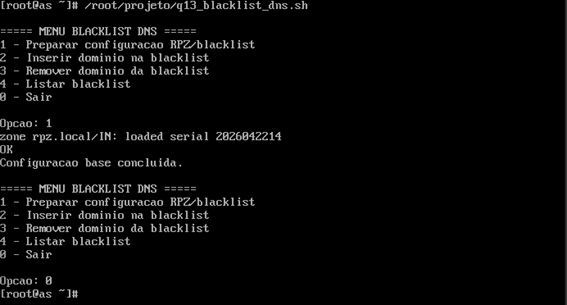
\includegraphics[width=0.78\textwidth,height=0.72\textheight,keepaspectratio]{figuras/q13_prep_menu.png}
}{
  \fbox{\parbox{0.9\textwidth}{Inserir screenshot da prepara\c{c}\~ao da configura\c{c}\~ao RPZ (op\c{c}\~ao 1).}}
}
\caption{Prepara\c{c}\~ao inicial da blacklist RPZ}
\label{fig:q13-prep}
\end{figure}

\begin{figure}[!htbp]
\centering
\IfFileExists{figuras/q13_response_policy.png}{
  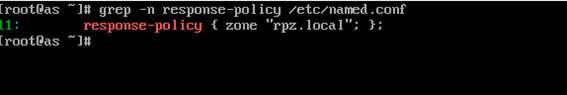
\includegraphics[width=0.78\textwidth,height=0.72\textheight,keepaspectratio]{figuras/q13_response_policy.png}
}{
  \fbox{\parbox{0.9\textwidth}{Inserir screenshot da diretiva \texttt{response-policy} no \texttt{/etc/named.conf}.}}
}
\caption{Valida\c{c}\~ao da diretiva \texttt{response-policy} no BIND}
\label{fig:q13-response-policy}
\end{figure}

\begin{figure}[!htbp]
\centering
\IfFileExists{figuras/q13_rpz_base_zone.png}{
  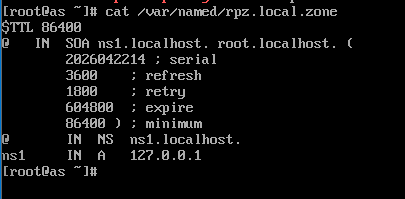
\includegraphics[width=0.78\textwidth,height=0.72\textheight,keepaspectratio]{figuras/q13_rpz_base_zone.png}
}{
  \fbox{\parbox{0.9\textwidth}{Inserir screenshot do conte\'udo inicial de \texttt{/var/named/rpz.local.zone}.}}
}
\caption{Ficheiro base da zona RPZ}
\label{fig:q13-rpz-base}
\end{figure}

\begin{figure}[!htbp]
\centering
\IfFileExists{figuras/q13_nslookup_before.png}{
  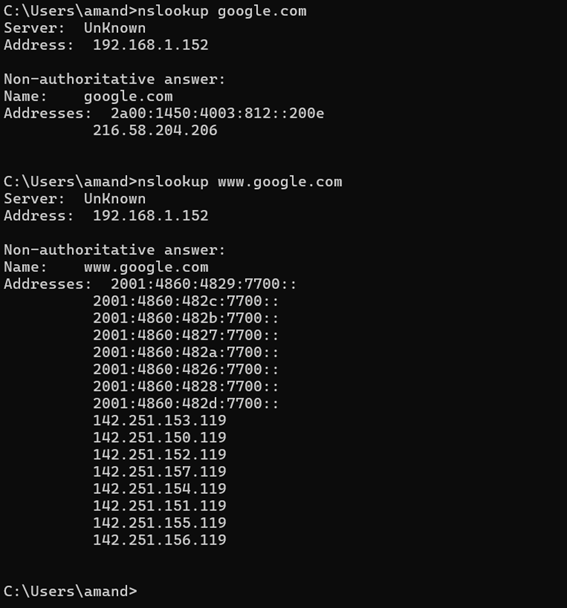
\includegraphics[width=0.78\textwidth,height=0.72\textheight,keepaspectratio]{figuras/q13_nslookup_before.png}
}{
  \fbox{\parbox{0.9\textwidth}{Inserir screenshot do \texttt{nslookup} antes da inser\c{c}\~ao na blacklist.}}
}
\caption{Resolu\c{c}\~ao normal antes da blacklist}
\label{fig:q13-before}
\end{figure}

\begin{figure}[!htbp]
\centering
\IfFileExists{figuras/q13_insert_list.png}{
  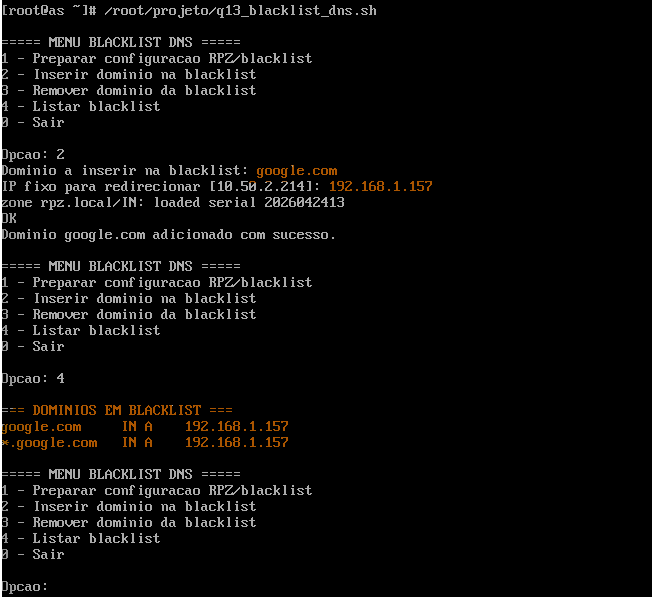
\includegraphics[width=0.78\textwidth,height=0.72\textheight,keepaspectratio]{figuras/q13_insert_list.png}
}{
  \fbox{\parbox{0.9\textwidth}{Inserir screenshot da inser\c{c}\~ao de dom\'inio e listagem da blacklist.}}
}
\caption{Inser\c{c}\~ao de \texttt{google.com} na blacklist}
\label{fig:q13-insert}
\end{figure}

\begin{figure}[!htbp]
\centering
\IfFileExists{figuras/q13_rpz_after_insert.png}{
  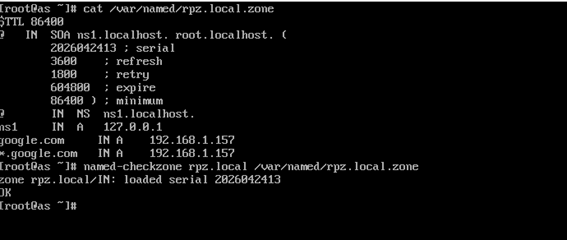
\includegraphics[width=0.78\textwidth,height=0.72\textheight,keepaspectratio]{figuras/q13_rpz_after_insert.png}
}{
  \fbox{\parbox{0.9\textwidth}{Inserir screenshot do ficheiro RPZ e valida\c{c}\~ao com \texttt{named-checkzone}.}}
}
\caption{Zona RPZ ap\'os inser\c{c}\~ao e valida\c{c}\~ao}
\label{fig:q13-zone-after}
\end{figure}

\begin{figure}[!htbp]
\centering
\IfFileExists{figuras/q13_nslookup_after.png}{
  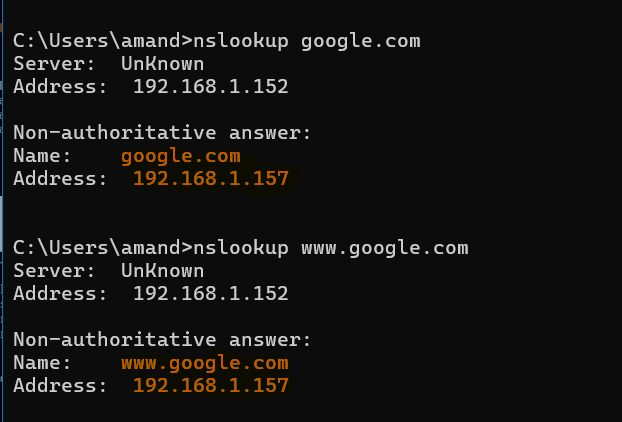
\includegraphics[width=0.78\textwidth,height=0.72\textheight,keepaspectratio]{figuras/q13_nslookup_after.png}
}{
  \fbox{\parbox{0.9\textwidth}{Inserir screenshot do \texttt{nslookup} ap\'os inser\c{c}\~ao na blacklist.}}
}
\caption{Resolu\c{c}\~ao redirecionada para IP fixo}
\label{fig:q13-after}
\end{figure}

\begin{figure}[!htbp]
\centering
\IfFileExists{figuras/q13_remove_list.png}{
  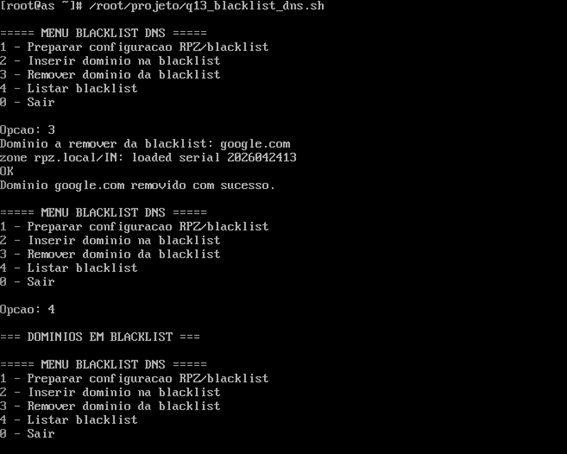
\includegraphics[width=0.78\textwidth,height=0.72\textheight,keepaspectratio]{figuras/q13_remove_list.png}
}{
  \fbox{\parbox{0.9\textwidth}{Inserir screenshot da remo\c{c}\~ao do dom\'inio e listagem final da blacklist.}}
}
\caption{Remo\c{c}\~ao do dom\'inio da blacklist}
\label{fig:q13-remove}
\end{figure}







